
\documentclass[a4paper,11pt]{article}
\usepackage[a4paper, margin=8em]{geometry}

% usa i pacchetti per la scrittura in italiano
\usepackage[french,italian]{babel}
\usepackage[T1]{fontenc}
\usepackage[utf8]{inputenc}
\frenchspacing 

% usa i pacchetti per la formattazione matematica
\usepackage{amsmath, amssymb, amsthm, amsfonts}

% usa altri pacchetti
\usepackage{gensymb}
\usepackage{hyperref}
\usepackage{standalone}

\usepackage{colortbl}

\usepackage{xstring}
\usepackage{karnaugh-map}

% imposta il titolo
\title{Appunti Calcolatori Elettronici}
\author{Luca Seggiani}
\date{2025}

% imposta lo stile
% usa helvetica
\usepackage[scaled]{helvet}
% usa palatino
\usepackage{palatino}
% usa un font monospazio guardabile
\usepackage{lmodern}

\renewcommand{\rmdefault}{ppl}
\renewcommand{\sfdefault}{phv}
\renewcommand{\ttdefault}{lmtt}

% circuiti
\usepackage{circuitikz}
\usetikzlibrary{babel}

% testo cerchiato
\newcommand*\circled[1]{\tikz[baseline=(char.base)]{
            \node[shape=circle,draw,inner sep=2pt] (char) {#1};}}

% disponi il titolo
\makeatletter
\renewcommand{\maketitle} {
	\begin{center} 
		\begin{minipage}[t]{.8\textwidth}
			\textsf{\huge\bfseries \@title} 
		\end{minipage}%
		\begin{minipage}[t]{.2\textwidth}
			\raggedleft \vspace{-1.65em}
			\textsf{\small \@author} \vfill
			\textsf{\small \@date}
		\end{minipage}
		\par
	\end{center}

	\thispagestyle{empty}
	\pagestyle{fancy}
}
\makeatother

% disponi teoremi
\usepackage{tcolorbox}
\newtcolorbox[auto counter, number within=section]{theorem}[2][]{%
	colback=blue!10, 
	colframe=blue!40!black, 
	sharp corners=northwest,
	fonttitle=\sffamily\bfseries, 
	title=Teorema~\thetcbcounter: #2, 
	#1
}

% disponi definizioni
\newtcolorbox[auto counter, number within=section]{definition}[2][]{%
	colback=red!10,
	colframe=red!40!black,
	sharp corners=northwest,
	fonttitle=\sffamily\bfseries,
	title=Definizione~\thetcbcounter: #2,
	#1
}

% disponi codice
\usepackage{listings}
\usepackage[table]{xcolor}

\definecolor{codegreen}{rgb}{0,0.6,0}
\definecolor{codegray}{rgb}{0.5,0.5,0.5}
\definecolor{codepurple}{rgb}{0.58,0,0.82}
\definecolor{backcolour}{rgb}{0.95,0.95,0.92}

\lstdefinestyle{codestyle}{
		backgroundcolor=\color{black!5}, 
		commentstyle=\color{codegreen},
		keywordstyle=\bfseries\color{magenta},
		numberstyle=\sffamily\tiny\color{black!60},
		stringstyle=\color{green!50!black},
		basicstyle=\ttfamily\footnotesize,
		breakatwhitespace=false,         
		breaklines=true,                 
		captionpos=b,                    
		keepspaces=true,                 
		numbers=left,                    
		numbersep=5pt,                  
		showspaces=false,                
		showstringspaces=false,
		showtabs=false,                  
		tabsize=2
}

\lstdefinestyle{shellstyle}{
		backgroundcolor=\color{black!5}, 
		basicstyle=\ttfamily\footnotesize\color{black}, 
		commentstyle=\color{black}, 
		keywordstyle=\color{black},
		numberstyle=\color{black!5},
		stringstyle=\color{black}, 
		showspaces=false,
		showstringspaces=false, 
		showtabs=false, 
		tabsize=2, 
		numbers=none, 
		breaklines=true
}


\lstdefinelanguage{assembler}{ 
  keywords={AAA, AAD, AAM, AAS, ADC, ADCB, ADCW, ADCL, ADD, ADDB, ADDW, ADDL, AND, ANDB, ANDW, ANDL,
        ARPL, BOUND, BSF, BSFL, BSFW, BSR, BSRL, BSRW, BSWAP, BT, BTC, BTCB, BTCW, BTCL, BTR, 
        BTRB, BTRW, BTRL, BTS, BTSB, BTSW, BTSL, CALL, CBW, CDQ, CLC, CLD, CLI, CLTS, CMC, CMP,
        CMPB, CMPW, CMPL, CMPS, CMPSB, CMPSD, CMPSW, CMPXCHG, CMPXCHGB, CMPXCHGW, CMPXCHGL,
        CMPXCHG8B, CPUID, CWDE, DAA, DAS, DEC, DECB, DECW, DECL, DIV, DIVB, DIVW, DIVL, ENTER,
        HLT, IDIV, IDIVB, IDIVW, IDIVL, IMUL, IMULB, IMULW, IMULL, IN, INB, INW, INL, INC, INCB,
        INCW, INCL, INS, INSB, INSD, INSW, INT, INT3, INTO, INVD, INVLPG, IRET, IRETD, JA, JAE,
        JB, JBE, JC, JCXZ, JE, JECXZ, JG, JGE, JL, JLE, JMP, JNA, JNAE, JNB, JNBE, JNC, JNE, JNG,
        JNGE, JNL, JNLE, JNO, JNP, JNS, JNZ, JO, JP, JPE, JPO, JS, JZ, LAHF, LAR, LCALL, LDS,
        LEA, LEAVE, LES, LFS, LGDT, LGS, LIDT, LMSW, LOCK, LODSB, LODSD, LODSW, LOOP, LOOPE,
        LOOPNE, LSL, LSS, LTR, MOV, MOVB, MOVW, MOVL, MOVSB, MOVSD, MOVSW, MOVSX, MOVSXB,
        MOVSXW, MOVSXL, MOVZX, MOVZXB, MOVZXW, MOVZXL, MUL, MULB, MULW, MULL, NEG, NEGB, NEGW,
        NEGL, NOP, NOT, NOTB, NOTW, NOTL, OR, ORB, ORW, ORL, OUT, OUTB, OUTW, OUTL, OUTSB, OUTSD,
        OUTSW, POP, POPL, POPW, POPB, POPA, POPAD, POPF, POPFD, PUSH, PUSHL, PUSHW, PUSHB, PUSHA, 
				PUSHAD, PUSHF, PUSHFD, RCL, RCLB, RCLW, MOVSL, MOVSB, MOVSW, STOSL, STOSB, STOSW, LODSB, LODSW,
				LODSL, INSB, INSW, INSL, OUTSB, OUTSL, OUTSW
        RCLL, RCR, RCRB, RCRW, RCRL, RDMSR, RDPMC, RDTSC, REP, REPE, REPNE, RET, ROL, ROLB, ROLW,
        ROLL, ROR, RORB, RORW, RORL, SAHF, SAL, SALB, SALW, SALL, SAR, SARB, SARW, SARL, SBB,
        SBBB, SBBW, SBBL, SCASB, SCASD, SCASW, SETA, SETAE, SETB, SETBE, SETC, SETE, SETG, SETGE,
        SETL, SETLE, SETNA, SETNAE, SETNB, SETNBE, SETNC, SETNE, SETNG, SETNGE, SETNL, SETNLE,
        SETNO, SETNP, SETNS, SETNZ, SETO, SETP, SETPE, SETPO, SETS, SETZ, SGDT, SHL, SHLB, SHLW,
        SHLL, SHLD, SHR, SHRB, SHRW, SHRL, SHRD, SIDT, SLDT, SMSW, STC, STD, STI, STOSB, STOSD,
        STOSW, STR, SUB, SUBB, SUBW, SUBL, TEST, TESTB, TESTW, TESTL, VERR, VERW, WAIT, WBINVD,
        XADD, XADDB, XADDW, XADDL, XCHG, XCHGB, XCHGW, XCHGL, XLAT, XLATB, XOR, XORB, XORW, XORL},
  keywordstyle=\color{blue}\bfseries,
  ndkeywordstyle=\color{darkgray}\bfseries,
  identifierstyle=\color{black},
  sensitive=false,
  comment=[l]{\#},
  morecomment=[s]{/*}{*/},
  commentstyle=\color{purple}\ttfamily,
  stringstyle=\color{red}\ttfamily,
  morestring=[b]',
  morestring=[b]"
}

\lstset{language=assembler, style=codestyle}

% disponi sezioni
\usepackage{titlesec}

\titleformat{\section}
	{\sffamily\Large\bfseries} 
	{\thesection}{1em}{} 
\titleformat{\subsection}
	{\sffamily\large\bfseries}   
	{\thesubsection}{1em}{} 
\titleformat{\subsubsection}
	{\sffamily\normalsize\bfseries} 
	{\thesubsubsection}{1em}{}

% tikz
\usepackage{tikz}

% float
\usepackage{float}

% grafici
\usepackage{pgfplots}
\pgfplotsset{width=10cm,compat=1.9}

% disponi alberi
\usepackage{forest}

\forestset{
	rectstyle/.style={
		for tree={rectangle,draw,font=\large\sffamily}
	},
	roundstyle/.style={
		for tree={circle,draw,font=\large}
	}
}

% disponi algoritmi
\usepackage{algorithm}
\usepackage{algorithmic}
\makeatletter
\renewcommand{\ALG@name}{Algoritmo}
\makeatother

% disponi numeri di pagina
\usepackage{fancyhdr}
\fancyhf{} 
\fancyfoot[L]{\sffamily{\thepage}}

\makeatletter
\fancyhead[L]{\raisebox{1ex}[0pt][0pt]{\sffamily{\@title \ \@date}}} 
\fancyhead[R]{\raisebox{1ex}[0pt][0pt]{\sffamily{\@author}}}
\makeatother

\begin{document}
% sezione (data)
\section{Lezione del 21-03-25}

% stili pagina
\thispagestyle{empty}
\pagestyle{fancy}

% testo
Andiamo a definire più nei dettagli la struttura di un processo e le modalità secondo le quali questi si possono creare e distruggere.

\subsection{Descrittori di processo}
Un processo è descritto fondalmente da un astrazione, detta \textbf{descrittore di processo}, idealmente contenuta in una qualche locazione contigua, assieme ad altri descrittori, in memoria.
Questo può essere schematizzato come una struttura C++ del tipo:
\begin{lstlisting}[language=C++, style=codestyle]	
struct des_proc {
	// identificatore numerico del processo
	natw id;
	// livello di privilegio (LIV_UTENTE o LIV_SISTEMA)
	natw livello;
	// precedenza nelle code dei processi
	natl precedenza;
	// indirizzo della base della pila sistema
	vaddr punt_nucleo;
	// copia dei registri generali del processore
	natq contesto[N_REG];

	// prossimo processo in coda
	des_proc* puntatore;

	// informazioni di debug
};
\end{lstlisting}
dove quindi si tiene conto di:
\begin{itemize}
	\item Un \textbf{indice} numerico unico ad ogni processo;
	\item Il \textbf{livello di privilegio} di un processo, che può essere \textit{utente} o \textit{sistema} (non è altro che la distinzione che avevamo fatto trattando la protezione di \textit{processi utente} e \textit{processi sistema});
	\item La \textbf{precedenza} del processo, la cui motivazione ci sarà chiara fra poco;
	\item Un puntatore alla \textbf{pila sistema} del processo;
	\item Il \textbf{contesto} del processo, inteso come la copia di tutti i registri del processore. 
	\item Infine, un puntatore al \textbf{prossimo processo}, in quanto intendiamo organizzare questi processi in linked liste ordinate per precedenza decrescente.
\end{itemize}

Ogni processo ha quindi un ciclo di vita che rispetta l'andamento del seguente grafico:
\begin{center}
	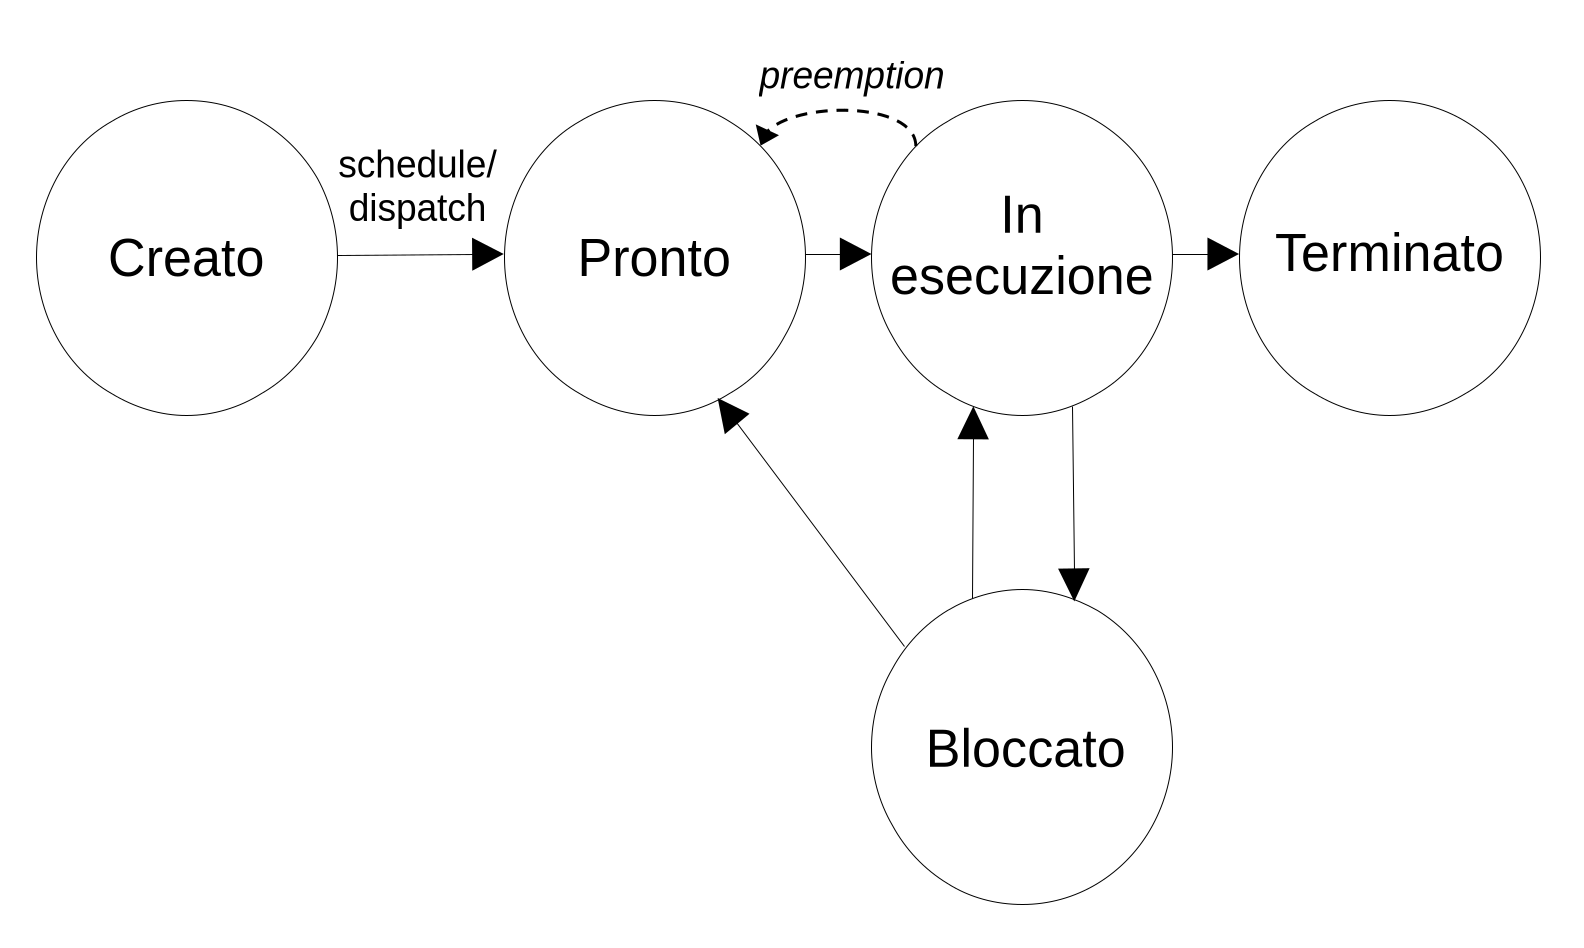
\includegraphics[scale=0.3]{../figures/schema_proc.png}
\end{center}

Vediamo nel dettaglio il significato delle diverse fasi.
In fase di creazione del proesso, il suo descrittore viene posto in una struttura dati che ne consente \textbf{schedulazione} e \textbf{dispatch}:
\begin{itemize}
	\item \textbf{Schedulazione:} effettivamente la scelta che il kernel fa, assunto il controllo, su qual'è il prossimo processo da portare in esecuzione (passaggio da processo \textbf{pronto} a processo in \textbf{esecuzione});
	\item \textbf{Dispatch:} l'esecuzione effettiva di una serie di operazioni di tale processo. 
\end{itemize}

I processi possono anche \textbf{bloccarsi}, cioè mettersi in attesa di qualche evento. 

Infine, un processo può \textbf{terminare}, cioè sparire dal sistema (lui e il suo descrittore).
Anche in questo caso il processo deve essere attualmente in esecuzione.

Una transizione che non è prevista da tutti i sistemi è quella di \textbf{preemption}, cioè di ritorno allo stato \textbf{pronto} a controllo dello scheduler.
La maggior parte dei sistemi operativi supporta tale funzionalità, il nucleo che vedremo solo parzialmente.

\subsubsection{Code di processi}
L'esistenza di processi bloccati e pronti richiede l'esistenza di una struttura dati che ne tenga conto.
Questa struttura dati, come abbiamo accennata, è rappresentata nel kernel studiato da linked list ordinate per precedenza decrescente.
Una lista viene definita per i processi pronti:
\begin{lstlisting}[language=C++, style=codestyle]	
// i processi pronti
des_proc* pronti;
\end{lstlisting}
mentre vedremo i processi bloccati lo sono in relazione a particolari oggetti, detti \textit{semafori}.

Notiamo quindi l'esistenza della variabile \lstinline|esecuzione|, che tiene conto del processo correntemente in esecuzione:
\begin{lstlisting}[language=C++, style=codestyle]	
// il processo in esecuzione (sempre 1)
des_proc* esecuzione;
\end{lstlisting}

Visto che bisognerà lavorare con liste di processi, si definiscono funzioni per la loro manipolazione:
\begin{itemize}
	\item \textbf{Inserimento di processo:} prende la forma di un semplice inserimento ordinato in lista.
\begin{lstlisting}[language=C++, style=codestyle]	
void inserimento_lista(des_proc*& p_lista, des_proc* p_elem)
{
// inserimento in una lista semplice ordinata
//   (tecnica dei due puntatori)
	des_proc *pp, *prevp;

	pp = p_lista;
	prevp = nullptr;
	while (pp && pp->precedenza >= p_elem->precedenza) {
		prevp = pp;
		pp = pp->puntatore;
	}

	p_elem->puntatore = pp;

	if (prevp)
		prevp->puntatore = p_elem;
	else
		p_lista = p_elem;

}
\end{lstlisting}
	\item \textbf{Rimozione di un processo:} prende la forma dell'estrazione della testa (cioè del processo a priorità più alta).
\begin{lstlisting}[language=C++, style=codestyle]	
des_proc* rimozione_lista(des_proc*& p_lista)
{
// estrazione dalla testa
	des_proc* p_elem = p_lista;  	// nullptr se la lista è vuota

	if (p_lista)
		p_lista = p_lista->puntatore;

	if (p_elem)
		p_elem->puntatore = nullptr;

	return p_elem;
}
\end{lstlisting}
\item \textbf{Inserzione forzata:} è usata in casi particolari, inserisce il processo corrente in testa alla lista ignorando il suo livello di precedenza.
	La motivazione di tale comportamento è quella di non "svantaggiare" inutilmente il processo corrente se, ad esempio, ne si è interrotta l'esecuzione con preemption per la gestione di un interruzinoe esterna.
\begin{lstlisting}[language=C++, style=codestyle]	
extern "C" void inspronti()
{
	esecuzione->puntatore = pronti;
	pronti = esecuzione;
}
\end{lstlisting}
\end{itemize}

\subsection{Prima vista dell'esecuzione del kernel}
Dopo il boot della macchina, il kernel si impadronisce della macchina e lancia il primo processo (il processo utente).
Da qui in poi il kernel avrà il controllo solo fra un processo e l'altro, in caso di interruzioni (interne, esterne o eccezioni), e potrà restituirlo solo attraverso il ritorno da gestore con \lstinline|IRETQ|.

Come abbiamo visto, ad ogni chiamata di gestore di interruzione lascia RIP, CS, RFLAGS e RSP al tempo di chiamata dell'interruzione (facendo le opportune distinzioni fra \textit{fault} e \textit{trap}) in pila.
A questo punto il gestore fa una copia dei registri generali, e si ha a quel punto una \textit{"foto"} del processore al momento di attraversamento del gate, che rappresenterà quindi il \textit{contesto} del processo stesso al momento della chiamata dell'interruzione.

In questo, sfrutteremo delle routine (\lstinline|salva_stato| e \lstinline|carica_stato|) all'avvio e al termine di ogni gestore, che si occupano di salvare e caricare il contesto del processo attualmente in esecuzione.
Per conoscere quale questo processo sia, sfruttiamo la variabile globale nel sistema introdotta prima, \lstinline|esecuzione|, che punta al descrittore del processo (che è dove vogliamo mettere il contesto stesso).

Un gestore di interruzione di base, quindi, si potrebbe magari occupare di passare al contesto e all'esecuzione del processo di priorità più alta a intervalli regolari, magari regolato da un timer (cosiddetto \textit{timeslicing}).

Altre situazioni, più vicine a noi, sono quelle del termine di una gestione di un interruzione esterna, o bloccaggio automatico di un processo, dove il kernel deve selezionare il prossimo processo da eseguire, scegliendo chiaramente quello a priorità più alta.

\subsubsection{Processo dummy}
Inseriamo un processo fittizio, \textit{dummy}, nella lista dei processi pronti con la priorità più bassa possibile.
Questo ci assicurerà di non trovarci mai una situazione dove nessun processo è pronto all'esecuzione, e quindi avere sempre qualcosa a cui il kernel può passare (idealmente il processo dummy effettua solo un ciclo a vuoto).

\subsubsection{Inizializzazione di un processo}
Un ulteriore dettaglio è quello dello stato del processo alla sua creazione.
Non è infatti realistico pensare di controllare se quel processo richiede inizializzazione ogni volta che si ritorna da un interruzione gestita a livello sistema.
Alla creazione del processo, quindi, vogliamo svolgere le seguenti azioni in modo che il processo venga eseguito per la prima volta già in uno stato completo:
\begin{itemize}
	\item Allocare una \textbf{pila sistema} dedicata al processo;
	\item Inizializzare la pila sistema. Questo consisterà nell'inizializzare a loro volta: 
		\begin{itemize}
			\item RIP alla prima istruzione del processo;
			\item CS al segmento livello utente dove si trova il processo;
			\item RFLAG a quanto viene richiesto dallo standard C++ al momento di avvio (solitamente tutto a 0), con l'eccezione di IF a 1.
		\end{itemize}
	\item Allocare il \textbf{descrittore} di processo, e mettere quel processo fra i processi pronti;
	\item Inizializzare il descrittore. Questo consiste nell'inizializzare a loro volta:
		\begin{itemize}
			\item Un puntatore alla pila sistema appena definita;
			\item Il contesto del processo;
			\item L'\textbf{argomento} di chiamata del processo, utile al debug;
			\item L'\textbf{IOPL}, \textit{IO Privilege Level}, che specifica la possibilità o meno del processo di accedere all'IO.
		\end{itemize}
\end{itemize}

\end{document}
